\section{Instance Layout}

\begin{figure}
    \begin{minipage}{.35\textwidth}
        \centering
        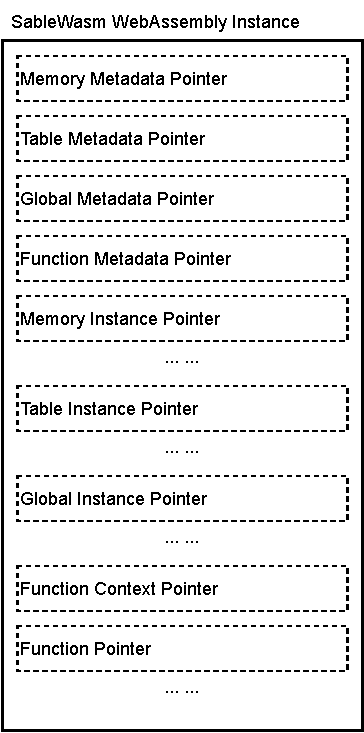
\includegraphics[width=\textwidth]{Images/5.Backend_and_Runtime/instance}
    \end{minipage}\hfill
    \begin{minipage}{.6\textwidth}
        \begin{lstlisting}[language=C, basicstyle=\ttfamily\footnotesize]
struct instance {
    memory_metadata_t   *memory_metadata;
    table_metadata_t    *table_metadata;
    global_metadata_t   *global_metadata;
    function_metadata_t *function_metadata;
    memory_t            *memories[NUM_MEMORY];
    table_t             *tables[NUM_TABLE];
    global_t            *globals[NUM_GLOBAL];
    struct {
        struct instance *context;
        function_t      *function_ptr;
    } * functions[NUM_FUNCTIONS];
};        
    \end{lstlisting}
    \end{minipage}
    \caption{SableWasm WebAssembly instance}
    \label{fig:backend-instance}
\end{figure}

This section discusses the WebAssembly instance implementation in SableWasm. A WebAssembly instance hosts all the runtime structures that the generated shared libraries require, such as linear memory and indirect table. Figure~\ref{fig:backend-instance} illustrates the design of the WebAssembly instance. SableWasm's WebAssembly instance consists of two parts, metadata entries and entity pointers. One may also notice that the instance object's size may vary from modules to modules depending on how many entities are declared. This behaviour is intensional by design. SableWasm runtime system needs to compute the address of the pointers based on the metadata information on the fly. By packing all pointers in a consecutive memory region, we reduce one layer of indirection for the runtime system, and in theory, may improve runtime performance. On the other hand, the generated shared library has all the entities address inlined as the backend can infer them during code generation, which does not incur any performance loss. For most of the entities, they are pretty straightforward, and we will skip the discussion here. In the rest of the section, we focus on three aspects: the metadata entries, the function entity representations, and the instance initialization protocol in SableWasm.

\paragraph{Metadata}
One could think of the metadata as the signatures for entities, and indeed, the SableWasm runtime system prepares the instance object based on the metadata. Further, shared libraries generated by SableWasm only publicly expose the metadata and initialization function to conceal module details. Metadata encodes the type for the entity. For linear memories and indirect tables, this is relatively trivial as their types only consist of an integer pair. In the case of global values, things are a little bit complicated. A quick reminder, WebAssembly global types keep track of their value type and mutability. The first problem here is how to encode WebAssembly value types. One solution is to use WebAssembly value type binary format. However, this encoding strategy emits hard to maintain results as a human can not directly read them. Here we use the JVM approach for value type encoding \footnote{\url{https://docs.oracle.com/javase/7/docs/technotes/guides/jni/spec/types.html}}. A quick summary, in SableWasm, we encode 32-bit integers as `I', 64-bit integers as 'J', single-precision floating-point number as 'F', double-precision floating-point number as 'D' and finally, 128-bit vector type as 'V'. The second problem is how to encode global's mutability. In SableWasm, we use capital letters for constant global value types and lower letters for mutable ones. Finally, for function types, we follow a similar design as we used for global values. SableWasm encodes function type into a null-terminated string. Let's take \texttt{[i32, f32] -> [v128]} as an example. SableWasm encodes the type into `\texttt{IF:V}'. The colon acts as a separator between parameter types and result types. Note that `\texttt{:}' itself is also a valid SableWasm function type string, and represents \texttt{[] -> []}, a void function with no arguments. Finally, metadata also encode module names and entity names for import entities and names for export entities, which play a critical role later in the module initialization phase.

\paragraph{Function entity representation}
WebAssembly specifications classify the functions into two groups, WebAssembly functions and host functions. WebAssembly functions are any functions defined within the module. On the other hand, the runtime system provides host functions to the module, and from the WebAssembly module point of view, the host functions are black boxes without any knowledge of their internals. Making things more complex, in MVP WebAssembly, there are no explicit requirements on how the WebAssembly functions should behave if they are invoked from other modules. Here we use a similar generalization like the one adopted by Javascript \footnote{WebAssembly Javascript Interface: \url{https://www.w3.org/TR/wasm-js-api-1/}}. In summary, in SableWasm, if a module exports a function, it exports the function in a closure that captures its enclosing instance. Suppose a second module invokes the exported closure via import functions. In that case, the function still only has access to its original module's entities and only communicates to the second module via return values. Hence, in SableWasm, we implement our function as a pair of pointers. The first one refers to its enclosing instance, and the second one relates to the generated function code. For host functions, we always set the enclosing instance pointer as a null pointer. In the chapter's introduction, we mentioned that we pass the instance object as the first argument to the generated functions upon function calls. But, what should we give to the host function invocations? SableWasm defines that for all the host functions, the instance object pointer will always point to the caller's enclosing instance instead of null so that the host functions can access the internals of the caller's module.

\paragraph{Initialization protocol}
In the last part of the section, we will cover the initialization protocol we used in SableWasm. The initialization protocol consists of three basic steps, validation, instance preparation and initialization. In the validation phase, we load the shared library with the operating system's help, such as \texttt{dlopen} in Linux, and check if it contains all the required symbols. Currently, a SableWasm shared library needs to export five symbols in total. Table~\ref{tbl:sablewasm-runtime-export-syms} illustrates the symbols expected from the generated shared libraries. The instance initializer function takes a prepared instance object as the argument. The next step in SableWasm is to construct this prepared instance object. The idea of a prepared instance object is that we want to separate the memory allocation from the value initialization. In SableWasm, the runtime system handles the memory allocation, while on the other hand, the initializer function takes care of the value initialization. In the second phase, the SableWasm runtime allocates all the entities and attaches them to the module instance. Note that SableWasm also resolves all the import names at this stage, and it will only proceed to the next step if all the expecting import entities are set. The import name binding utilizes the module names and entity names provided by the metadata. Finally, the last step is the initialization. SableWasm will invoke the initializer function supplied by the shared library. The initializer function takes care of all kinds of value initialization, such as setting values for global variables and copy data segments into linear memory. If the runtime system adequately prepares the instance context, the initializer function should never fail.

\begin{table}[h]
    \centering
    \begin{tabular}{|l|l|}
        \hline
        \textbf{Symbol Name}          & \textbf{Description}          \\ \hline
        \_\_sable\_global\_metadata   & Metadata for global values    \\ \hline
        \_\_sable\_memory\_metadata   & Metadata for linear memories  \\ \hline
        \_\_sable\_table\_metadata    & Metadata for indirect tables  \\ \hline
        \_\_sable\_function\_metadata & Metadata for functions        \\ \hline
        \_\_sable\_initialize         & Instance initializer function \\ \hline
    \end{tabular}
    \caption{SableWasm shared libraries exported symbols}
    \label{tbl:sablewasm-runtime-export-syms}
\end{table}